\documentclass[a4paper,11pt]{report}
\usepackage{chuan_math_gkt}
\usetikzlibrary{angles,quotes,intersections,patterns,decorations.pathreplacing}
\chuanexamsetup

\begin{document}
\examfontsize

\examsecret{绝密$\bigstar$启用前}

\examtitle{2026年普通高等学校招生全国统一考试（北京卷）}{数\quad 学}

\noticetitle
\begin{examnotice}
\item 答卷前，考生务必将自己的姓名、准考证号填写在答题卡上. 
\item 回答选择题时，选出每小题的答案后，用铅笔把答题卡上对应题目的答案标号涂黑. 如需改动，用橡皮擦干净后，再选涂其他答案标号. 回答非选择题时，将答案写在答题卡上. 写在本试卷上无效. 
\item 考试结束后，将本试卷和答题卡一并交回. 
\end{examnotice}

\examsection{一、选择题：本题共10小题，每小题4分，共40分. 在每小题给出的四个选项中，只有一项符合题目要求.}
\begin{examquestions}
\item 已知集合 $M=\{x\mid -1<x<3\}$，$N=\{x\mid x\geq2\}$，则 $M\cup N=$
\fourchoices{$(2,3)$}{$(-1,+\infty)$}{$[2,3)$}{$(-1,2]$}

\item 已知 $z_1=3-2\mathrm{i}$，$z_2=-1+4\mathrm{i}$，则 $|z_1+z_2|=$
\fourchoices{$2\sqrt2$}{$\mathrm{i}$}{$2$}{$8$}

\item 已知双曲线 $C:\dfrac{x^2}{a^2}-\dfrac{y^2}{4}=1(a>0)$ 的渐近线方程为 $y=\pm\dfrac23x$，则 $a$ 的值为
\fourchoices{$2$}{$3$}{$4$}{$9$}

\item 已知 $(a-\sqrt{x})^7$ 的展开式中的 $x^2$ 的系数是 $280$，则 $a=$
\fourchoices{$2$}{$-2$}{$1$}{$-1$}

\item 下列函数 $f(x)$ 是奇函数且在定义域上单调递增的是
\twochoices
{$f(x)=\dfrac1{x^2+1}$}
{$f(x)=\sin x$}
{$f(x)=2^{-x}-2^x$}
{$f(x)=\ln\dfrac{5+x}{5-x}$}

\item 已知向量 $\vec a,\vec b$ 满足 $|\vec a-\vec b|=2$，$\vec a=(2,0)$，则 $|\vec b|$ 的最大值为
\fourchoices{$1$}{$2$}{$3$}{$4$}

\item $\{a_n\},\{b_n\}$ 是无穷数列，则“存在常数 $M$，使 $a_n\leq M\leq b_n(n=1,2,3,\cdots)$”是“$a_n\leq b_n(n=1,2,3,\cdots)$”的
\twochoices
{充分不必要条件}
{必要不充分条件}
{充要条件}
{既不充分也不必要条件}

\item 已知 $f(x)=\sin(x+\varphi)(0<\varphi<2\pi)$，将 $f(x)$ 向 $x$ 轴正方向平移 $3\varphi$ 个单位，得到的函数图象与 $f(x)$ 图象关于 $x$ 轴对称，则 $\varphi$ 的取值个数为
\fourchoices{$1$}{$2$}{$3$}{$4$}

\item 学校组织高一、高二学生参观甲、乙两地博物馆，每位学生可自主选择一处前往. 已知高一学生总人数多于高二学生总人数，前往甲地的全体学生总数多于前往乙地的全体学生总数，则
\onechoices
{去甲地的高一学生人数多于去乙地的高一学生人数}
{去甲地的高一学生人数多于去乙地的高二学生人数}
{去甲地的高一学生人数不多于去乙地的高二学生人数}
{去乙地的高二学生人数不少于去甲地的高二学生人数}


\item 有如图所示的播杆机械装置，其中 $A,B$ 为定点，$C,D$ 是动点，$AD=1$，$CD=3$，$BC=\dfrac52$，$AB=4$，则 $\cos\angle ABC$ 的取值范围为

\noindent\begin{minipage}[t]{0.7\linewidth}
\twochoices
{\tallchoice{$\left[\dfrac5{16},\dfrac{73}{80}\right]$}}
{\tallchoice{$\left[-\dfrac5{16},\dfrac{73}{80}\right]$}}
{\tallchoice{$\left[\dfrac5{16},1\right]$}}
{\tallchoice{$\left[\dfrac5{16},\dfrac{73}{80}\right)$}}
\end{minipage}\hfill
\begin{minipage}[t]{0.28\linewidth}
\vspace{-1em}
\centering
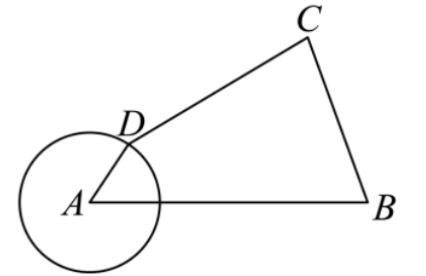
\includegraphics[width=\linewidth]{figures/2026_bj_q10.png}
\end{minipage}


\end{examquestions}

\examsection{二、填空题：本题共5小题，每小题5分，共25分.}
\begin{examquestions}[start=11]
\item 已知直线 $ax+y=0$ 与圆 $(x-2)^2+(y-2)^2=4$ 相切，则 $a=$ \blank.

\item 已知等差数列 $\{a_n\}$ 的前 $n$ 项和为 $S_n$，且 $S_6=6a_6+30$，则公差 $d=$ \blank，若 $S_n\leq S_5$ 恒成立，则符合条件的 $a_1$ 的一个取值为 \blank.

\item 音高 $y$（单位：mel）与频率 $f$（单位：Hz）满足 $y=\lg\left(1+\dfrac{f}{700}\right)$，若 $\lg2\leq y\leq3\lg2$，则 $f$ 的取值范围为 \blank.

\noindent\begin{minipage}[t]{0.7\linewidth}
\item 已知三棱锥 $A-BCD$，$AB=AC=AD=2\sqrt2$，$BC=BD=2$，$CD=2\sqrt3$，则底面 $BCD$ 的面积为 \blank；体积为 \blank.
\end{minipage}\hfill
\begin{minipage}[t]{0.26\linewidth}
\vspace{-1.2em}
\centering
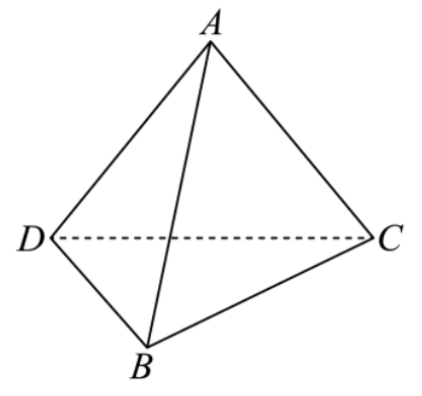
\includegraphics[width=\linewidth]{figures/2026_bj_q14.png}
\end{minipage}
\vspace{-2em}
\item 已知 $f(x)=\left|x^2-\cos x-c^2\right|$，给出下列四个结论：

\gktcircled{1} $f(x)$ 在 $(-1,1)$ 上有最小值和最大值；

\gktcircled{2} 当 $c=0$ 时，$f(x)=1$ 有 $3$ 个解；

\gktcircled{3} 当 $c=1$，$x\in(-1,2]$ 时，$f(x)$ 有最大值；

\gktcircled{4} 当 $c>0$ 时，$f(x)$ 与 $y=c$ 有 $4$ 个交点.

其中正确结论的序号是 \blank.
\end{examquestions}

\examsection{四、解答题：本题共6小题，共85分. 解答应写出文字说明、证明过程或演算步骤.}
\begin{examanswers}[start=16]
\item（13分）

已知函数 $f(x)=2\sin\omega x\cos\varphi+2\cos\omega x\sin\varphi$，$\omega>0$，$|\varphi|<\dfrac{\pi}{2}$，$f(x)$ 的最小正周期为 $\pi$，且 $f(0)>0$，$f\left(\dfrac{\pi}{4}\right)=1$.

\subq{（1）}{求 $\omega,\varphi$ 的值；}

\subq{（2）}{求 $f(x)$ 的单调递减区间.}

\item（13分）

现从全校学生中随机抽取 $200$ 人统计数学成绩，成绩分组及对应人数如下：

\begin{tightcenter}
{\renewcommand{\arraystretch}{0.9}
\begin{tabular}{c|ccccc}
\hline
成绩分组 & $[81,94)$ & $[94,107)$ & $[107,120)$ & $[120,135)$ & $[135,150]$\\
\hline
人数 & $40$ & $60$ & $60$ & $32$ & $8$\\
\hline
\end{tabular}}
\end{tightcenter}

以频率估计概率，完成下列问题：

\subq{（1）}{求数学成绩低于 $120$ 的概率；}

\subq{（2）}{从学校随机抽取 $4$ 人，求 $2$ 人分数不低于 $120$ 且 $2$ 人分数小于 $94$ 的概率；}

\subq{（3）}{每组数据取左端、中间、右端，比较 $s^2_{\text{左}},s^2_{\text{中}},s^2_{\text{右}}$ 的大小关系.}

\item（14分）

已知直三棱柱 $ABC-A_1B_1C_1$，$\angle BAC=90^\circ$，$AB=AC=2$，$BB_1=\sqrt2$，$D,E$ 分别为棱 $A_1B_1,AC$ 的中点.

\noindent\begin{minipage}[t]{0.64\linewidth}
\subq{（1）}{证明：$DE\parallel$ 平面 $BB_1C_1C$；}

\subq{（2）}{点 $P$ 在平面 $A_1B_1C_1$ 内，且 $EP\parallel B_1C_1$，再从条件\gktcircled{1}、条件\gktcircled{2}、条件\gktcircled{3}这三个条件中选择一个作为已知，使得点 $P$ 唯一确定，求平面 $PAD$ 与平面 $PDE$ 的夹角的余弦值.

条件\gktcircled{1}：$PA=PD$；

条件\gktcircled{2}：$PA\perp BC$；

条件\gktcircled{3}：$BB_1\parallel$ 平面 $PDE$.

注：如果选择条件\gktcircled{1}、条件\gktcircled{2}、条件\gktcircled{3}分别解答，按第一个解答计分.
}
\end{minipage}\hfill
\begin{minipage}[t]{0.3\linewidth}
\vspace{-1.0em}
\centering
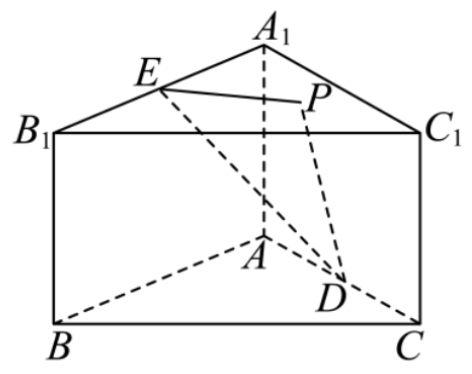
\includegraphics[width=\linewidth]{figures/2026_bj_q18.png}
\end{minipage}
\newpage
\item（15分）

已知椭圆 $E:\dfrac{x^2}{a^2}+\dfrac{y^2}{b^2}=1(a>b>0)$ 的一个顶点是 $(2,0)$，离心率为 $\dfrac12$.

\subq{（1）}{求 $E$ 的方程；}

\subq{（2）}{过点 $A(1,1)$，斜率为 $k(k\neq\pm1)$ 的直线交椭圆 $E$ 于 $B,C$ 两点，$B$ 关于 $y=x$ 的对称点为 $D$，直线 $CD$ 交 $y=x$ 于点 $Q$，若 $|S_{\triangle ABQ}-S_{\triangle ACQ}|=\dfrac58$，求 $k$.}

\item（15分）

设函数 $f(x)=x^2+mx-4e^{nx-1}(n\in\mathbb Z)$，曲线 $y=f(x)$ 在点 $(-1,f(-1))$ 处的切线方程为 $4x+e^2y+e^2+8=0$.

\subq{（1）}{求 $m,n$ 的值；}

\subq{（2）}{求 $f(x)$ 的极值点的个数；}

\subq{（3）}{求 $y=kx-1(k>0)$ 的图象与 $f(x)$ 的图象的交点个数.}

\item（15分）

设 $A=(a_{ij})_{m\times n}$ 是一个 $m$ 行 $n$ 列的数阵，且数阵中的每一项 $a_{ij}\in\{-1,1\}$. 若对任意 $1\leq i,p\leq m$，$1\leq j,q\leq n$，其中 $i\neq p$，$j\neq q$，$||i-p|-|j-q||=2$，都有 $a_{ij}+a_{iq}+a_{pj}+a_{pq}=0$，则称数阵 $A$ 具有性质 $P$.

\subq{（1）}{判断下列两个数表是否具有性质 $P$：
\begin{tightcenter}
\begin{tabular}{c|cccc}
\hline
$A_1$ & $1$ & $1$ & $-1$ & $1$\\
     & $-1$ & $1$ & $-1$ & $1$\\
\hline
$A_2$ & $1$ & $1$ & $-1$ & $-1$\\
     & $1$ & $-1$ & $1$ & $-1$\\
     & $-1$ & $1$ & $-1$ & $1$\\
\hline
\end{tabular}
\end{tightcenter}
}

\subq{（2）}{在所有具有性质 $P$ 的 $5\times4$ 数阵中，$1$ 的个数最多是多少；}

\subq{（3）}{若 $m=n=6$，$a_{11}=1$，且数阵 $A$ 具有性质 $P$，证明：对任意 $i,j\in\{1,2,3,4,5,6\}$，都有 $a_{ij}=a_{1i}a_{1j}$.}
\end{examanswers}

\end{document}